%%%%%%%%%%%%%%%%%%%%%%%%%%%%%%%%%%%%%%%%%
%----------------------------------------------------------------------------------------
%	PACKAGES AND OTHER DOCUMENT CONFIGURATIONS
%----------------------------------------------------------------------------------------

\documentclass{article}

%%%%%%%%%%%%%%%%%%%%%%%%%%%%%%%%%%%%%%%%%
% Lachaise Assignment
% Structure Specification File
% Version 1.0 (26/6/2018)
%
% This template originates from:
% http://www.LaTeXTemplates.com
%
% Authors:
% Marion Lachaise & François Févotte
% Vel (vel@LaTeXTemplates.com)
%
% License:
% CC BY-NC-SA 3.0 (http://creativecommons.org/licenses/by-nc-sa/3.0/)
% 
%%%%%%%%%%%%%%%%%%%%%%%%%%%%%%%%%%%%%%%%%

%----------------------------------------------------------------------------------------
%	PACKAGES AND OTHER DOCUMENT CONFIGURATIONS
%----------------------------------------------------------------------------------------

\usepackage{amsmath,amsfonts,stmaryrd,amssymb} % Math packages

\usepackage{enumerate} % Custom item numbers for enumerations

\usepackage[ruled]{algorithm2e} % Algorithms

\usepackage[framemethod=tikz]{mdframed} % Allows defining custom boxed/framed environments

\usepackage{listings} % File listings, with syntax highlighting
\lstset{
	basicstyle=\ttfamily, % Typeset listings in monospace font
}

%----------------------------------------------------------------------------------------
%	DOCUMENT MARGINS
%----------------------------------------------------------------------------------------

\usepackage{geometry} % Required for adjusting page dimensions and margins

\geometry{
	paper=a4paper, % Paper size, change to letterpaper for US letter size
	top=2.5cm, % Top margin
	bottom=3cm, % Bottom margin
	left=2.5cm, % Left margin
	right=2.5cm, % Right margin
	headheight=14pt, % Header height
	footskip=1.5cm, % Space from the bottom margin to the baseline of the footer
	headsep=1.2cm, % Space from the top margin to the baseline of the header
	%showframe, % Uncomment to show how the type block is set on the page
}

%----------------------------------------------------------------------------------------
%	FONTS
%----------------------------------------------------------------------------------------

\usepackage[utf8]{inputenc} % Required for inputting international characters
\usepackage[T1]{fontenc} % Output font encoding for international characters

\usepackage{XCharter} % Use the XCharter fonts

%----------------------------------------------------------------------------------------
%	COMMAND LINE ENVIRONMENT
%----------------------------------------------------------------------------------------

% Usage:
% \begin{commandline}
%	\begin{verbatim}
%		$ ls
%		
%		Applications	Desktop	...
%	\end{verbatim}
% \end{commandline}

\mdfdefinestyle{commandline}{
	leftmargin=10pt,
	rightmargin=10pt,
	innerleftmargin=15pt,
	middlelinecolor=black!50!white,
	middlelinewidth=2pt,
	frametitlerule=false,
	backgroundcolor=black!5!white,
	frametitle={Command Line},
	frametitlefont={\normalfont\sffamily\color{white}\hspace{-1em}},
	frametitlebackgroundcolor=black!50!white,
	nobreak,
}

% Define a custom environment for command-line snapshots
\newenvironment{commandline}{
	\medskip
	\begin{mdframed}[style=commandline]
}{
	\end{mdframed}
	\medskip
}

%----------------------------------------------------------------------------------------
%	FILE CONTENTS ENVIRONMENT
%----------------------------------------------------------------------------------------

% Usage:
% \begin{file}[optional filename, defaults to "File"]
%	File contents, for example, with a listings environment
% \end{file}

\mdfdefinestyle{file}{
	innertopmargin=1.6\baselineskip,
	innerbottommargin=0.8\baselineskip,
	topline=false, bottomline=false,
	leftline=false, rightline=false,
	leftmargin=2cm,
	rightmargin=2cm,
	singleextra={%
		\draw[fill=black!10!white](P)++(0,-1.2em)rectangle(P-|O);
		\node[anchor=north west]
		at(P-|O){\ttfamily\mdfilename};
		%
		\def\l{3em}
		\draw(O-|P)++(-\l,0)--++(\l,\l)--(P)--(P-|O)--(O)--cycle;
		\draw(O-|P)++(-\l,0)--++(0,\l)--++(\l,0);
	},
	nobreak,
}

% Define a custom environment for file contents
\newenvironment{file}[1][File]{ % Set the default filename to "File"
	\medskip
	\newcommand{\mdfilename}{#1}
	\begin{mdframed}[style=file]
}{
	\end{mdframed}
	\medskip
}

%----------------------------------------------------------------------------------------
%	NUMBERED QUESTIONS ENVIRONMENT
%----------------------------------------------------------------------------------------

% Usage:
% \begin{question}[optional title]
%	Question contents
% \end{question}

\mdfdefinestyle{question}{
	innertopmargin=1.2\baselineskip,
	innerbottommargin=0.8\baselineskip,
	roundcorner=5pt,
	nobreak,
	singleextra={%
		\draw(P-|O)node[xshift=1em,anchor=west,fill=white,draw,rounded corners=5pt]{%
		Question \theQuestion\questionTitle};
	},
}

\newcounter{Question} % Stores the current question number that gets iterated with each new question

% Define a custom environment for numbered questions
\newenvironment{question}[1][\unskip]{
	\bigskip
	\stepcounter{Question}
	\newcommand{\questionTitle}{~#1}
	\begin{mdframed}[style=question]
}{
	\end{mdframed}
	\medskip
}

%----------------------------------------------------------------------------------------
%	WARNING TEXT ENVIRONMENT
%----------------------------------------------------------------------------------------

% Usage:
% \begin{warn}[optional title, defaults to "Warning:"]
%	Contents
% \end{warn}

\mdfdefinestyle{warning}{
	topline=false, bottomline=false,
	leftline=false, rightline=false,
	nobreak,
	singleextra={%
		\draw(P-|O)++(-0.5em,0)node(tmp1){};
		\draw(P-|O)++(0.5em,0)node(tmp2){};
		\fill[black,rotate around={45:(P-|O)}](tmp1)rectangle(tmp2);
		\node at(P-|O){\color{white}\scriptsize\bf !};
		\draw[very thick](P-|O)++(0,-1em)--(O);%--(O-|P);
	}
}

% Define a custom environment for warning text
\newenvironment{warn}[1][Warning:]{ % Set the default warning to "Warning:"
	\medskip
	\begin{mdframed}[style=warning]
		\noindent{\textbf{#1}}
}{
	\end{mdframed}
}

%----------------------------------------------------------------------------------------
%	INFORMATION ENVIRONMENT
%----------------------------------------------------------------------------------------

% Usage:
% \begin{info}[optional title, defaults to "Info:"]
% 	contents
% 	\end{info}

\mdfdefinestyle{info}{%
	topline=false, bottomline=false,
	leftline=false, rightline=false,
	nobreak,
	singleextra={%
		\fill[black](P-|O)circle[radius=0.4em];
		\node at(P-|O){\color{white}\scriptsize\bf i};
		\draw[very thick](P-|O)++(0,-0.8em)--(O);%--(O-|P);
	}
}

% Define a custom environment for information
\newenvironment{info}[1][Info:]{ % Set the default title to "Info:"
	\medskip
	\begin{mdframed}[style=info]
		\noindent{\textbf{#1}}
}{
	\end{mdframed}
}
 % Inclde the file specifying the document structure and custom commands
\usepackage{float}
%----------------------------------------------------------------------------------------
%	ASSIGNMENT INFORMATION
%----------------------------------------------------------------------------------------

\title{CALIFORNIA STATE UNIVERSITY, FRESNO    \\DEPARTMENT OF COMPUTER SCIENCE} % Title of the assignment

%----------------------------------------------------------------------------------------

\begin{document}

\maketitle % Print the title
\begin{tabular}{|c|c|c|c|c|c|}
	\hline 
	Class: & \multicolumn{3}{c|}{Big Data Analytic (CSCI 191T)} & Semester: & Spring 2020 \\ 
	\hline 
	\multicolumn{6}{|c|}{} \\ 
	\hline 
	Points &  & Document author: & \multicolumn{3}{c|}{Leonardo Yoshida} \\ 
	\hline 
	&  & Author's email: & \multicolumn{3}{c|}{yoshida\_leoy@mail.fresnostate.edu} \\ 
	\hline 
	&  & Assignment number: & \multicolumn{3}{c|}{3} \\ 
	\hline 
	\multicolumn{6}{|c|}{} \\ 
	\hline 
\end{tabular} 

%----------------------------------------------------------------------------------------
%	INTRODUCTION
%----------------------------------------------------------------------------------------

\section{Statement of Objectives}

The objective of this assignment was to perform descriptive analysis on two datasets, one personal and provided. The main significance of this assignment was to interpret the visualizations created using matplotlib and determine the type of distribution each dataset had for a specific variable.

\section{Experimental Procedure} % Numbered section

For this experiment, the tools utilized were python, pandas, numpy and matplotlib . The experiments was performed in a windows machine with intel-i7 processor and 16GB of RAM and on a linux machine with intel-i7 and 8GB of ram. Both yielded the same results. The datasets used were about movie metadata, movie ratings and US accidents and their impact onf traffic.

%------------------------------------------------

\subsection{Procedure}

The first step of the experiment was to load the datasets into the python program. To do that I used the read\_csv function provided by the pandas library. Once the datasets were loaded, I used the info, head and describe functions also provided by pandas to get a basic understanding of the datasets. For the movies metadata dataset, i had to remove rows that had a budget value of 0, since they would interfere with the analysis. To do that, first i converted the values of the row to numeric using the to\_numeric function provided pandas. The function converted the strings into numbers with the exception of some specific values that could not be converted. To deal with does values I added the parameter errors='coerce' to the function and this transformed those values into NaN. Once the data was transformed to numeric and NaN, i used the dropna function to remove all rows that had budget equal to NaN and then took a subset of the data removing rows with budget equal to 0. Once that was complete i utilized the mean and var functions to find the mean and variance of the budget column. For the movie ratings and US accidents I did not need to go through the cleaning step since the columns I was going to analyze were already clean. For these datasets, I simply selected the column I was going to analyze and used the function value\_counts() to create a set of key value pairs where the key was the variable and the value was the number of occurrences. Once I had that, Iu used the matplotlib library to plot a pie chart and a histogram to visualize their distribution.


\section{Analysis}

Discuss and justify the experimental results. Insert the chart or graph of your results to back up your analysis.
\subsection{Movies MetaData}
After analyzing the budget column of the movies metadata dataset, I was able to find its mean and variance. Those were equal to 21604277.457480315 and 1177219164512387.5 respectively. By looking at these numbers we can clearly see that most data points in the dataset seem to be far different from the mean, showing there is a big variation when it comes to a movies budget.

\begin{figure}[H]
	\centering
	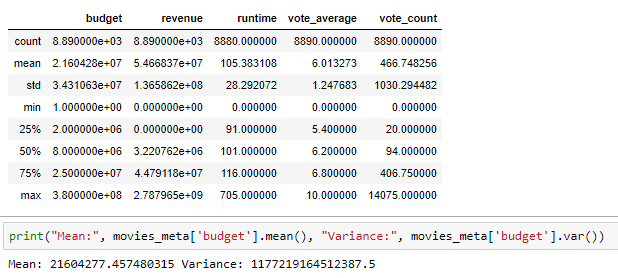
\includegraphics{moivie_meta}
	\caption{Descriptive analysis of the data}
\end{figure}

\subsection{Movie Ratings}
By looking at both the pie chart and histogram on Figure2, we can see most of the ratings are between 3 and 4. If we look at the shape of the histogram, I believe the most probable distribution that can be applied to this graph is a Gaussean distribution. However, because of technical problems with python, I was not able to plot the distribution line.
\begin{figure}[H]
	\centering
	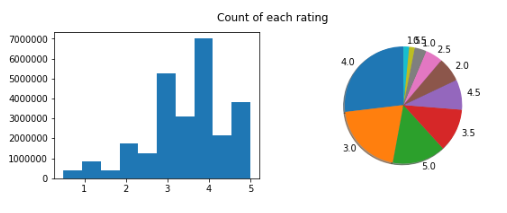
\includegraphics{movie rating}
	\caption{Histogram and pie chart showing distribution of movie ratings}
\end{figure}


\subsection{Personal Dataset: US Accidents}
By looking at both the pie chart and histogram on Figure3, we can see most of the accident types are of type 2. If we look at the shape of the histogram, I believe the most probable distribution that can be applied to this graph is a Exponential distribution since the amount of accidents seem to decrease exponentially the higher the type. However, because of technical problems with python, I was not able to plot the distribution line.
\begin{figure}[H]
	\centering
	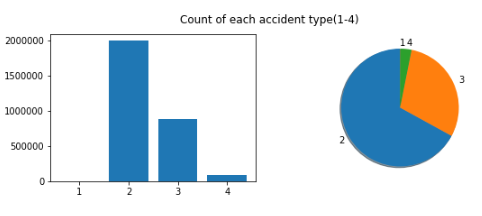
\includegraphics{accident}
	\caption{Histogram and pie chart showing distribution of US accidents}
\end{figure}


\section{Encountered Problems}
As mentioned before I had some trouble with the distribution line. My problem was mostly on how to calculate it. I researched several possible libraries to help me solve this problem such as scipy and seaborne however none of the solutions I found helped me

\section{Conclusions}
In conclusion, by doing this experiment I learned several things. First, i got better used to plotting graphs using matplotlib and pandas. By plotting different types of graphs, i got a better understanding of the different graphs that can be created using the library. Second, I got a better understanding of descriptive analysis by performing it on different datasets. Finally I grasped a better understanding on how to identify distribution types by analyzing means, variances and the shape of graphs.

\section{References}

https://www.kaggle.com/rounakbanik/the-movies-dataset/version/7 \\
https://www.kaggle.com/sobhanmoosavi/us-accidents


\end{document}
